\chapter{LRDE Presentation}


\section{Line of business}
The \LRDE\space (Research and Development Laboratory of \EPITA) is focused on fundamental
research and development in computer science. Its main areas of expertise are:
\begin{itemize}
 \item Image processing and pattern recognition
 \item Automata and verification
 \item Performance and genericity
\end{itemize}


\noindent Building on its solid scientific production and academic collaborations, the laboratory has
industrial contracts, conducts internal research projects and participates in collaborative
academic research projects.

\noindent Its members also give classes to students at \EPITA.

\section{The Laboratory}
The \LRDE\space (\url{https://www.lrde.epita.fr/wiki/Home}) was created in February 1998 to promote
the research activity at \EPITA\space and to allow students to be involved into important research
projects.

The research activity at \LRDE\space is focusing on subjects related to the school with the aim
of getting recognition in the scientific domain through publications and by working together with other
research centers.\\
One particularity of the \LRDE\space is the will to create a bond between traditional
teaching given to \EPITA\space students and teaching through research. The point of this is to:
\begin{itemize}
  \item participate to the production of knowledge in computer science and to
	promote the image of \EPITA\space in scientific domain.
  \item develop \LRDE\space student's formation through research and allow them to access a third cycle
	formation.
\end{itemize}


\section{Members}
The laboratory is composed of a dozen permanent members, including teacher-researchers, engineers,
administration and PhD students. Each year, these permanent members recruit third year students
from \EPITA\space, whom will stay until the end of their studies, following a dedicated study specialisation
at \EPITA\space. Hence, the laboratory hosts two generations of students that can grow to a number
between ten to fifteen.


\section{Services}
The \LRDE\space is working on four different axis, all of which are represented by a project.


\subsection{Olena}
\begin{center}
 
\includegraphics[width=2cm]{img/olena.jpg}
\end{center}
The Olena project (\url{https://olena.lrde.epita.fr}) consists of a generic image processing library.
Its objective is to implement a platform of numerical scientific computations dedicated to image
processing, pattern recognition and computer vision. This environment is composed of a generic and
efficient library (Milena), a set of tools for shell scripts and a visual programming interface.
The project aims at offering an interpreted environment like MatLab or Mathematica.

Each of these parts imply its own difficulties and require the development of new solutions.
For example, the library, which require the entirety of low level features on which it relies on to be
both efficient and generic --- two objectives that are hard to meet at the same time in programmation.
Fortunately, the object oriented programming eases this problem if we avoid the classical object
modeling with inheritance and polymorphism. Hence, this genericity allows the development of efficient
and re-usable code. The Olena platform uses this paradigm. The project already addressed the problem
of the diversity of data and data structures.

Furthermore, the people working on this project were able to put in light the existence of conception
models related to generic programmation. Olena is an open source project under GPL license.


\subsection{\VCSN}
\begin{center}
 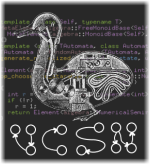
\includegraphics[width=2cm]{img/vcsn.png}
\end{center}
The \VCSN project (\url{https://vcsn.lrde.epita.fr}) is a finite state machine manipulation
platform developed in collaboration with the ENST. Finite state machines, also called automata,
are useful for language treatment and task automation. In the past, such platforms, like "FSM",
were supposed to work for problems of industrial scale. Hence, for efficiency reasons, they were
specialized in letter automata. On the other hand, platforms like "FSA" were based on a more abstract
approach. \VCSN tries to answer both of these issues by using techniques of static and generic
programmation in C++.

\VCSN can then support the entirety of automata with multiplicity in any kind of
semiring. Thanks to generic programming techniques, it is not necessary to code a single algorithm once
for each type of automata anymore. A single abstract version is sufficient, and this without loosing
efficiency. It is not necessary to handle C++ perfectly to be able to use the platform thanks to an
interpreter conceived to highlight all of the system's potential. This environment should allow
researchers to experiment their ideas and beginners to practice with an intuitive interface.

\VCSN is an open source project under GPL license.


\subsection{Spot}
\begin{center}
 
\includegraphics[width=2cm]{img/spot.png}
\end{center}
Spot (\url{https://spot.lrde.epita.fr/}) is a library of algorithms for "model checking",
which is a way to check that every possible behavior of a system satisy its given properties.
Spot allows to express those properties using temporal logic. It corresponds to classical propositional
calculus (with its "or", "and" and "not" operators) equiped with temporal operators to express things
such as "in a future time" or "anytime since now". Such formula can be translated to automata
(Spot implements different algorithms), such that verifying that the behavior of a model satisfy a
formula can be reduced to operations between two automata (here again Spot implements different
algorithms).

This approach can be applied to different kind of systems: communication protocoles,
electronic circuits, programs...


\subsection{Speaker ID}
The Speaker Recognition team is working on Machine Learning solutions applied to Speaker Recognition
tasks. They propose statistical representations of speech signal which are more robust to the problem
of session and channel variabilities. They participated in the evaluation campaign of speaker
verification systems organized by NIST (the National Institute of Standards and Technology) which
organizes competitions in various fields, both to stimulate research and to define new standards since
the beginning of the project.


\section{The internship in the company's work}